\section{Introducción}

\subsection{Área temática}
\begin{frame}{Área temática}
	Este trabajo se basa en 5 pilares teóricos:
	\begin{itemize} [<+>]
		\item Sitios de Community Question Answering (CQA).
		\item Medidas de similaridad.
		\item Sistemas de Recomendación.
		\item Big Data.
		\item Ensamble de Clustering.
	\end{itemize}
\end{frame}

\subsection{Tema específico}
\begin{frame}[allowframebreaks]{Tema específico}
	\begin{figure}
		\centering
		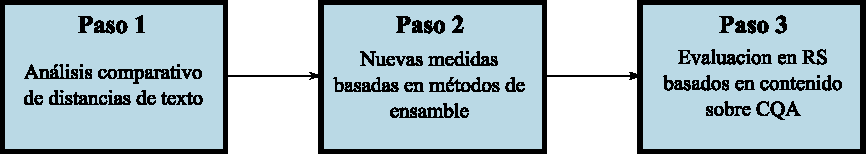
\includegraphics[width=0.7\linewidth]{../5_introduccion/imagenes/pipeline}
		\label{fig:pipeline}

		\framebreak

		Considerando el conjunto completo de datos Quora (\(404301\) pares de preguntas, es decir, \(808602\) preguntas totales), deberiamos realizar:

		\bigskip $\frac{n(n+1)}{2} = 326919001503$ calculos de distancias, donde $n = 808602$
	\end{figure}
\end{frame}

\subsection{Objetivo general}
\begin{frame}{Objetivo general}
	Construir una arquitectura Big Data que incluye la posibilidad de ser aplicada a grandes conjuntos de datos de preguntas en el ámbito de CQA y, a partir de esta arquitectura, implementar y evaluar nuevas medidas de similaridad entre textos que puedan ser utilizadas en sistemas de recomendación.
\end{frame}

\subsection{Objetivos específicos}
\begin{frame}{Objetivos específicos}
	\scriptsize
	\begin{itemize} [<+>]
		\item Diseñar y desarrollar una arquitectura Big Data para cálculo de similaridad en grandes matrices, que requerirá nuevas estrategias para recolectar, procesar y manejar grandes volúmenes de datos.
		\item Identificar medidas de similaridad de texto existentes y un método efectivo de aplicación de las mismas en grandes volúmenes de datos.
		\item Evaluar el comportamiento de medidas de similaridad de texto del estado del arte respecto al manejo del volumen, variedad, velocidad y veracidad inherentes a grandes volúmenes de datos, en particular en el ámbito de CQA.
		\item Proponer una nueva medida que permita integrar las medidas de similaridad del estado del arte mediante una arquitectura de software basada en Big Data y que sea extensible a otras medidas existentes en el estado del arte.
		\item Brindar conclusiones, pautas y recomendaciones para trabajar con medidas de comparación de textos en grandes volúmenes de datos en sitios de CQA utilizando arquitecturas basadas en Big Data.
	\end{itemize}
\end{frame}